\documentclass{article}

% ---------------------------------------------------------
% 1. SETUP & PACKAGES
% ---------------------------------------------------------
\PassOptionsToPackage{numbers, compress}{natbib}

% [preprint] shows your names. Change to [final] for the final version.
\usepackage[final]{neurips_2024}

% Remove the conference footer from the first page
\makeatletter
\renewcommand{\@noticestring}{}
\makeatother

\usepackage[utf8]{inputenc} % allow utf-8 input
\usepackage[T1]{fontenc}    % use 8-bit T1 fonts
\usepackage[french, provide=*]{babel}  % French language support
\usepackage{hyperref}       % hyperlinks
\usepackage{url}            % simple URL typesetting
\usepackage{booktabs}       % professional-quality tables
\usepackage{amsmath}        % best math environment
\usepackage{amsthm}         % for theorems
\newtheorem{theorem}{Théorème}
\usepackage{amsfonts}       % blackboard math symbols
\usepackage{nicefrac}       % compact symbols for 1/2, etc.
\usepackage[expansion=false]{microtype}      % microtypography
\usepackage{graphicx}       % for images
\usepackage{enumitem}       % for cleaner lists
\usepackage{multirow}
\usepackage{xcolor}         % color text
\usepackage{tikz}
\usetikzlibrary{shapes.geometric, arrows.meta, positioning, calc, decorations.pathreplacing}
\usepackage{pgfplots}
\pgfplotsset{compat=1.18}

% Custom Colors
\definecolor{myBlue}{RGB}{70, 130, 180}
\definecolor{myOrange}{RGB}{255, 140, 0}
\definecolor{myGreen}{RGB}{60, 179, 113}


% ---------------------------------------------------------
% 2. TITLE & AUTHORS
% ---------------------------------------------------------
\title{IWAE vs VAE : Borne Plus Serrée, Latents Plus Riches ?}

\author{%
  Amine Mike El Maalouf \\
  \texttt{amine.el-maalouf@epita.fr} \\
  \And
  Cedric Damais \\
  \texttt{cedric.damais@epita.fr} \\
  \And
  Yacine Benihaddadene \\
  \texttt{yacine.benihaddadene@epita.fr} \\
  \And
  Leon Ayral \\
  \texttt{leon.ayral@epita.fr} \\
  \And
  Oscar Le Dauphin \\
  \texttt{oscar.le-dauphin@epita.fr} \\
}

\begin{document}

\maketitle

% ---------------------------------------------------------
% 3. ABSTRACT
% ---------------------------------------------------------

\begin{abstract}
Les Autoencodeurs Variationnels (VAE) sont des modèles génératifs permettant d'approximer des distributions a posteriori complexes via la maximisation d'une borne inférieure variationnelle (ELBO). Cependant, l'objectif standard du VAE contraint souvent le modèle à apprendre des représentations simplifiées, limitant ainsi sa capacité de modélisation. Ce projet étudie l'Importance Weighted Autoencoder (IWAE), une généralisation du VAE qui optimise une borne strictement plus fine dérivée de l'échantillonnage préférentiel. Nous analysons l'impact théorique de cet objectif sur l'estimation des gradients et la flexibilité du postérieur. Nos expériences sur le jeu de données MNIST démontrent que l'utilisation de multiples échantillons pondérés ($K>1$) améliore significativement la log-vraisemblance par rapport au VAE standard ($K=1$). De plus, nos résultats confirment que l'IWAE exploite plus efficacement l'espace latent, augmentant le nombre d'unités actives et produisant des représentations plus riches. Cependant, nous étudions également une limitation critique : lorsque $K$ augmente, le rapport signal sur bruit (SNR) des gradients de l'encodeur diminue, dégradant potentiellement la capacité d'apprentissage de celui-ci.
\end{abstract}

\newpage
% ---------------------------------------------------------
% 4. SECTIONS
% ---------------------------------------------------------
\section{Introduction}

Les modèles génératifs profonds sont devenus un pilier de l'apprentissage automatique moderne, permettant la synthèse de données complexes telles que des images, du texte et de l'audio. Parmi ceux-ci, l'Autoencodeur Variationnel (VAE) \cite{kingma2013auto} se distingue comme une approche rigoureuse combinant réseaux de neurones et inférence bayésienne. En apprenant une correspondance probabiliste entre les observations et un espace latent structuré, les VAE offrent un cadre puissant pour la génération et l'apprentissage de représentations.

Cependant, l'objectif standard du VAE présente des limitations inhérentes. La borne inférieure sur l'évidence (ELBO) que les VAE maximisent peut être une approximation lâche de la vraie log-vraisemblance lorsque le postérieur approché $q_\phi(z|x)$ ne parvient pas à correspondre au vrai postérieur $p_\theta(z|x)$. Ce relâchement conduit à des phénomènes tels que l'\textbf{effondrement du postérieur} (posterior collapse), où le modèle ignore les dimensions latentes informatives et s'appuie entièrement sur le décodeur.

L'Importance Weighted Autoencoder (IWAE), introduit par \citet{burda2015importance}, répond à cette limitation en utilisant l'échantillonnage préférentiel pour obtenir une borne strictement plus serrée sur la log-vraisemblance. Dans ce rapport, nous étudions les fondements théoriques de l'IWAE, comparons ses performances au VAE standard sur le jeu de données MNIST, et explorons à la fois ses avantages et ses inconvénients potentiels. Nous examinons également les développements récents de la recherche qui ont construit sur le cadre de l'IWAE.

% ---------------------------------------------------------
\section{Contexte Théorique}

\subsection{L'Objectif : Inférence de Variables Latentes}

Étant donné des données observées $x$, notre objectif est d'apprendre la distribution a posteriori des variables latentes $z$ :
\begin{equation}
    p_\theta(z|x) = \frac{p_\theta(x|z)p(z)}{p_\theta(x)}
\end{equation}

où :
\begin{itemize}
    \item $p_\theta(x|z)$ : La vraisemblance (décodeur) paramétrée par $\theta$
    \item $p(z)$ : La distribution a priori (typiquement $\mathcal{N}(0,I)$)
    \item $p_\theta(x)$ : La vraisemblance marginale (évidence)
\end{itemize}

\paragraph{Le Problème de l'Intractabilité.} Le calcul direct du postérieur est intractable car la vraisemblance marginale nécessite une intégrale sur tout l'espace latent :
\begin{equation}
    p_\theta(x) = \int p_\theta(x|z)p(z) \, dz
\end{equation}

Pour des décodeurs de type réseau de neurones complexes, cette intégrale n'a pas de solution analytique. L'inférence variationnelle résout ce problème en approximant $p_\theta(z|x)$ par une distribution tractable $q_\phi(z|x)$ (l'encodeur), paramétrée par $\phi$.

\subsection{VAE Standard : L'Objectif ELBO}

Le VAE maximise la borne inférieure sur l'évidence (ELBO), qui fournit une borne inférieure sur la log-vraisemblance :
\begin{equation}
    \log p_\theta(x) \geq \mathcal{L}_{\text{VAE}} = \mathbb{E}_{z \sim q_\phi(z|x)} \left[ \log \frac{p_\theta(x,z)}{q_\phi(z|x)} \right]
\end{equation}

Cette borne peut être décomposée en :
\begin{equation}
    \mathcal{L}_{\text{VAE}} = \mathbb{E}_{q_\phi(z|x)}[\log p_\theta(x|z)] - \text{KL}(q_\phi(z|x) \| p(z))
\end{equation}

L'écart entre la vraie log-vraisemblance et l'ELBO est précisément la divergence KL entre les postérieurs approché et vrai :
\begin{equation}
    \log p_\theta(x) - \mathcal{L}_{\text{VAE}} = \text{KL}(q_\phi(z|x) \| p_\theta(z|x))
\end{equation}

Lorsque le postérieur approché $q_\phi(z|x)$ est trop simple (par exemple, une gaussienne diagonale) pour capturer le vrai postérieur, la borne devient lâche. Ce relâchement contribue au risque d'\textbf{effondrement du postérieur}, où le terme KL domine et le modèle apprend à ignorer le code latent.

% ---------------------------------------------------------
\section{La Solution IWAE}

L'Importance Weighted Autoencoder (IWAE) \cite{burda2015importance} répond au relâchement de l'ELBO en utilisant l'échantillonnage préférentiel avec $K$ échantillons au lieu d'un seul.

\subsection{L'Objectif IWAE}

L'objectif IWAE est défini comme :
\begin{equation}
    \mathcal{L}_K = \mathbb{E}_{z_1, \ldots, z_K \sim q_\phi(z|x)} \left[ \log \frac{1}{K} \sum_{i=1}^{K} w_i \right]
\end{equation}

où les poids d'importance sont :
\begin{equation}
    w_i = \frac{p_\theta(x, z_i)}{q_\phi(z_i|x)}
\end{equation}

Chaque poids $w_i$ mesure à quel point l'échantillon $z_i$ explique bien les données $x$ sous le modèle génératif, relativement à sa probabilité d'être échantillonné depuis l'encodeur.

\subsection{Nouveauté 1 : Bornes Strictement Plus Serrées}

\begin{theorem}[Burda et al., 2015]
La borne IWAE $\mathcal{L}_K$ est monotonement croissante avec $K$ :
\begin{equation}
    \mathcal{L}_1 \leq \mathcal{L}_2 \leq \cdots \leq \mathcal{L}_K \leq \cdots \leq \log p_\theta(x)
\end{equation}
\end{theorem}

La nouvelle borne découlant de l'inégalité de Jensen appliquée à la fonction logarithme concave :
\begin{equation}
    \mathbb{E} \left[ \log \left( \frac{1}{K} \sum_{i=1}^K w_i \right) \right] \leq \log \left( \mathbb{E} \left[ \frac{1}{K} \sum_{i=1}^K w_i \right] \right) = \log p_\theta(x)
\end{equation}

\textbf{Implications :}
\begin{itemize}
    \item Lorsque $K \to \infty$, l'estimateur converge vers la vraie vraisemblance marginale $\log p_\theta(x)$.
    \item Même avec un $K$ fini, nous obtenons un objectif garanti meilleur (plus serré) que le VAE standard qui utilise $K=1$.
\end{itemize}

\subsubsection{Démonstration: Borne monotonement croissante}
Voici la preuve mathématique que la borne IWAE est monotonement croissante avec $K$ :

Soit $I \subset \{1, \dots, k\}$ avec $|I| = m$ un sous-ensemble uniformément distribué d'indices distincts de $\{1, \dots, k\}$. Nous utiliserons l'observation simple suivante : $\mathbb{E}_{I=\{i_1, \dots, i_m\}} \left[ \frac{a_{i_1} + \dots + a_{i_m}}{m} \right] = \frac{a_1 + \dots + a_k}{k}$ pour toute suite de nombres $a_1, \dots, a_k$.

En utilisant cette observation et l'inégalité de Jensen, nous obtenons :

\begin{align}
\mathcal{L}_k &= \mathbb{E}_{\mathbf{h}_1, \dots, \mathbf{h}_k} \left[ \log \frac{1}{k} \sum_{i=1}^k \frac{p(\mathbf{x}, \mathbf{h}_i)}{q(\mathbf{h}_i|\mathbf{x})} \right] \tag{17} \\
&= \mathbb{E}_{\mathbf{h}_1, \dots, \mathbf{h}_k} \left[ \log \mathbb{E}_{I=\{i_1, \dots, i_m\}} \left[ \frac{1}{m} \sum_{j=1}^m \frac{p(\mathbf{x}, \mathbf{h}_{i_j})}{q(\mathbf{h}_{i_j}|\mathbf{x})} \right] \right] \tag{18} \\
&\geq \mathbb{E}_{\mathbf{h}_1, \dots, \mathbf{h}_k} \left[ \mathbb{E}_{I=\{i_1, \dots, i_m\}} \left[ \log \frac{1}{m} \sum_{j=1}^m \frac{p(\mathbf{x}, \mathbf{h}_{i_j})}{q(\mathbf{h}_{i_j}|\mathbf{x})} \right] \right] \tag{19} \\
&= \mathbb{E}_{\mathbf{h}_1, \dots, \mathbf{h}_m} \left[ \log \frac{1}{m} \sum_{i=1}^m \frac{p(\mathbf{x}, \mathbf{h}_i)}{q(\mathbf{h}_i|\mathbf{x})} \right] = \mathcal{L}_m \tag{20}
\end{align}



\subsection{Nouveauté 2 : Postérieurs Implicites Plus Riches}

L'objectif IWAE induit une distribution a posteriori implicite qui peut être plus complexe que $q_\phi(z|x)$. Les poids d'importance normalisés agissent comme un filtre :
\begin{equation}
    \tilde{w}_i = \frac{w_i}{\sum_{j=1}^K w_j}
\end{equation}

Le postérieur implicite peut s'écrire :
\begin{equation}
    \tilde{q}(z|x) \approx \sum_{i=1}^K \tilde{w}_i \delta(z - z_i)
\end{equation}

Cette représentation en mélange permet à l'IWAE de capturer des postérieurs multimodaux même lorsque la proposition de base $q_\phi(z|x)$ est unimodale. La mise à jour du gradient pour l'IWAE est :
\begin{equation}
    \nabla \mathcal{L}_K = \mathbb{E}_{\epsilon} \left[ \sum_{i=1}^{K} \tilde{w}_i \nabla_{\theta,\phi} \log w(x, z_i, \theta, \phi) \right]
\end{equation}

Les échantillons avec des poids normalisés élevés $\tilde{w}_i$ dominent la mise à jour du gradient, filtrant efficacement les ``mauvais'' échantillons qui expliquent mal les données.

\subsection{Pourquoi Échantillonner Plus Aide}

L'intuition clé derrière la robustesse de l'IWAE réside dans l'effet ``filet de sécurité'' de l'utilisation de multiples échantillons :

\textbf{Cas $K=1$ (Risqué) :} Si nous tirons un seul mauvais échantillon $z_1$ où $p_\theta(x,z_1)$ est très faible :
\begin{equation}
    w_1 \approx 0 \quad \Rightarrow \quad \log(w_1) \to -\infty
\end{equation}
Cela conduit à des gradients explosifs et un entraînement instable.

\textbf{Cas $K > 1$ (Couverture) :} Même si la plupart des échantillons sont mauvais, tant qu'un échantillon est bon :
\begin{equation}
    \log(0 + 0 + \cdots + w_{\text{bon}}) \approx \log(w_{\text{bon}}) > -\infty
\end{equation}

La somme agit comme un filet de sécurité, permettant à l'encodeur de faire des erreurs tant qu'il produit occasionnellement de bons échantillons.

% ---------------------------------------------------------
\section{Le Problème du SNR : Pourquoi un Grand K Nuit à l'Encodeur}
\label{sec:snr_problem}

Bien qu'augmenter $K$ fournisse une borne plus serrée sur la log-vraisemblance, cela s'accompagne d'un compromis critique : \textbf{la capacité d'apprentissage de l'encodeur se dégrade lorsque $K$ augmente}. Ce phénomène est lié au rapport signal sur bruit (SNR) de l'estimateur de gradient.

\subsection{Décomposition du Gradient}

L'objectif IWAE implique à la fois les paramètres génératifs $\theta$ (décodeur) et les paramètres d'inférence $\phi$ (encodeur). Le gradient par rapport à $\phi$ peut s'écrire en utilisant l'astuce de reparamétrisation \cite{kingma2013auto} :
\begin{equation}
    \nabla_\phi \mathcal{L}_K = \mathbb{E}_{\epsilon_1, \ldots, \epsilon_K} \left[ \sum_{i=1}^{K} \tilde{w}_i \nabla_\phi \log w(x, z_i(\phi, \epsilon_i), \theta, \phi) \right]
\end{equation}

où $z_i = \mu_\phi(x) + \sigma_\phi(x) \odot \epsilon_i$ avec $\epsilon_i \sim \mathcal{N}(0, I)$.

\subsection{Le Paradoxe du SNR}

Lorsque $K \to \infty$, quelque chose de contre-intuitif se produit. Considérons les poids normalisés $\tilde{w}_i$ :

\begin{itemize}
    \item À mesure que $K$ augmente, la distribution des poids d'importance devient plus concentrée : typiquement un échantillon aura $\tilde{w}_i \approx 1$ tandis que tous les autres auront $\tilde{w}_j \approx 0$.
    \item La mise à jour du gradient est dominée par le seul échantillon ``gagnant''.
    \item Cet échantillon gagnant est de plus en plus déterminé par \textbf{l'a priori $p(z)$ et la vraisemblance $p_\theta(x|z)$}, et non par la qualité de l'encodeur $q_\phi(z|x)$.
\end{itemize}

Mathématiquement, lorsque $K \to \infty$, l'objectif IWAE approche :
\begin{equation}
    \mathcal{L}_\infty = \log p_\theta(x) = \log \mathbb{E}_{z \sim q_\phi}[w(x, z)]
\end{equation}

À cette limite, l'objectif dépend de l'encodeur \textbf{uniquement à travers son support}, pas sa distribution spécifique. Tant que $q_\phi(z|x) > 0$ partout où $p_\theta(x,z) > 0$, la borne est exacte. Cela signifie que le signal de gradient pour $\phi$ disparaît.

\subsection{Analyse du Rapport Signal sur Bruit}

Le SNR du gradient de l'encodeur peut être défini comme :
\begin{equation}
    \text{SNR}(\nabla_\phi \mathcal{L}_K) = \frac{|\mathbb{E}[\nabla_\phi \mathcal{L}_K]|}{\text{Std}[\nabla_\phi \mathcal{L}_K]}
\end{equation}

\citet{rainforth2018tighter} ont montré que tandis que le SNR pour le décodeur $\theta$ \textbf{augmente} avec $K$, le SNR pour l'encodeur $\phi$ \textbf{diminue} avec $K$ :
\begin{equation}
    \text{SNR}(\nabla_\phi \mathcal{L}_K) = \mathcal{O}(K^{-1/2})
\end{equation}

Cela signifie que bien que nous obtenions une meilleure estimation de la log-vraisemblance, l'encodeur reçoit des signaux de gradient de plus en plus bruités et faibles.

\subsection{Implications Pratiques}

Cette dégradation du SNR a des conséquences importantes :
\begin{itemize}
    \item \textbf{Le décodeur apprend bien :} Le modèle génératif $p_\theta(x|z)$ continue de s'améliorer avec un $K$ plus grand.
    \item \textbf{L'encodeur peut stagner :} Le réseau d'inférence $q_\phi(z|x)$ reçoit des signaux de gradient diminuants et peut échouer à s'améliorer.
    \item \textbf{Un K optimal existe :} Il y a typiquement une valeur optimale de $K$ qui équilibre la borne plus serrée contre la capacité d'apprentissage de l'encodeur.
\end{itemize}

Cette analyse suggère que simplement augmenter $K$ n'est pas toujours bénéfique. L'objectif IWAE crée une asymétrie où le décodeur bénéficie de plus d'échantillons tandis que l'encodeur en souffre.

% ---------------------------------------------------------
\section{Méthodologie}

\subsection{Configuration Expérimentale}

Nous comparons le VAE ($K=1$) avec l'IWAE ($K>1$) en utilisant des architectures identiques pour assurer une comparaison équitable.

\begin{table}[h]
    \centering
    \begin{tabular}{l|c}
        \toprule
        \textbf{Paramètre} & \textbf{Valeur} \\
        \midrule
        Jeu de données & MNIST (Binarisé) \\
        Encodeur & MLP ($784 \to 200 \to 200 \to 50$) \\
        Décodeur & MLP ($50 \to 200 \to 200 \to 784$) \\
        Optimiseur & Adam ($lr=1\times10^{-3}$) \\
        Dimension Latente & 50 \\
        \textbf{K (Échantillons)} & \textbf{1, 5, 20, 30, 50, 100} \\
        \bottomrule
    \end{tabular}
    \caption{Configuration expérimentale}
\end{table}

\textbf{Détail d'Implémentation :} Nous utilisons \texttt{torch.logsumexp} pour calculer l'objectif IWAE, évitant le dépassement de capacité numérique lors du traitement de produits de nombreuses petites probabilités.

% ---------------------------------------------------------
\section{Résultats}

\subsection{Estimation de la Log-Vraisemblance}

La Figure~\ref{fig:loglikelihood} montre la log-vraisemblance estimée sur l'ensemble de test MNIST pour différentes valeurs de $K$.

\begin{figure}[h]
    \centering
    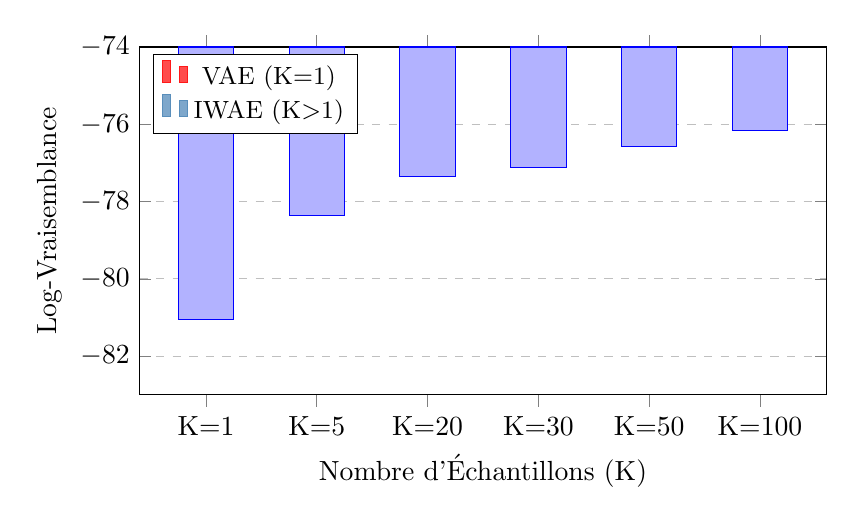
\begin{tikzpicture}
        \begin{axis}[
            ybar,
            width=0.85\textwidth,
            height=6cm,
            ylabel={Log-Vraisemblance},
            xlabel={Nombre d'Échantillons (K)},
            symbolic x coords={K=1, K=5, K=20, K=30, K=50, K=100},
            xtick=data,
            ymin=-83,
            ymax=-74,
            nodes near coords,
            nodes near coords align={vertical},
            every node near coord/.append style={font=\scriptsize},
            bar width=20pt,
            enlarge x limits=0.12,
            legend style={at={(0.02,0.98)}, anchor=north west, font=\small},
            ymajorgrids=true,
            grid style=dashed,
            scatter,
            scatter src=explicit symbolic,
            scatter/classes={
                vae={fill=red!70, draw=red!90},
                iwae={fill=myBlue!70, draw=myBlue!90}
            },
        ]
        \addplot coordinates {
            (K=1, -81.06) [vae]
            (K=5, -78.36) [iwae]
            (K=20, -77.34) [iwae]
            (K=30, -77.12) [iwae]
            (K=50, -76.58) [iwae]
            (K=100, -76.17) [iwae]
        };
        \addlegendimage{fill=red!70, draw=red!90, area legend}
        \addlegendentry{VAE (K=1)}
        \addlegendimage{fill=myBlue!70, draw=myBlue!90, area legend}
        \addlegendentry{IWAE (K$>$1)}
        \end{axis}
    \end{tikzpicture}
    \caption{Log-Vraisemblance Estimée sur l'Ensemble de Test MNIST (Plus Élevé = Mieux)}
    \label{fig:loglikelihood}
\end{figure}

\textbf{Observation :} Comme prédit par la théorie, $\mathcal{L}_{100} > \mathcal{L}_{50} > \mathcal{L}_{20} > \mathcal{L}_{5} > \mathcal{L}_{1}$. Augmenter $K$ resserre strictement la borne, améliorant l'estimation de la log-vraisemblance d'environ 5 nats de $K=1$ à $K=100$.

\subsection{Unités Latentes Actives}

Pour mesurer l'utilisation de l'espace latent, nous comptons les \textbf{unités actives} : dimensions latentes où la divergence KL dépasse un seuil $\epsilon = 0.01$.

\begin{figure}[h]
    \centering
    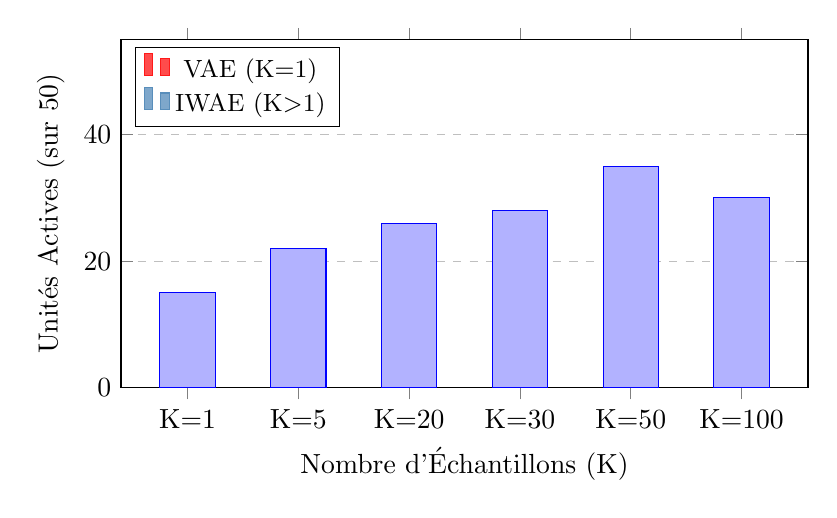
\begin{tikzpicture}
        \begin{axis}[
            ybar,
            width=0.85\textwidth,
            height=6cm,
            ylabel={Unités Actives (sur 50)},
            xlabel={Nombre d'Échantillons (K)},
            symbolic x coords={K=1, K=5, K=20, K=30, K=50, K=100},
            xtick=data,
            ymin=0,
            ymax=55,
            nodes near coords,
            nodes near coords align={vertical},
            every node near coord/.append style={font=\scriptsize},
            bar width=20pt,
            enlarge x limits=0.12,
            legend style={at={(0.02,0.98)}, anchor=north west, font=\small},
            ymajorgrids=true,
            grid style=dashed,
            scatter,
            scatter src=explicit symbolic,
            scatter/classes={
                vae={fill=red!70, draw=red!90},
                iwae={fill=myBlue!70, draw=myBlue!90}
            },
        ]
        \addplot coordinates {
            (K=1, 15) [vae]
            (K=5, 22) [iwae]
            (K=20, 26) [iwae]
            (K=30, 28) [iwae]
            (K=50, 35) [iwae]
            (K=100, 30) [iwae]
        };
        \addlegendimage{fill=red!70, draw=red!90, area legend}
        \addlegendentry{VAE (K=1)}
        \addlegendimage{fill=myBlue!70, draw=myBlue!90, area legend}
        \addlegendentry{IWAE (K$>$1)}
        \end{axis}
    \end{tikzpicture}
    \caption{Nombre de Dimensions Latentes Actives (Plus Élevé = Mieux)}
    \label{fig:activeunits}
\end{figure}

\textbf{Observation :} L'IWAE utilise plus de dimensions latentes que le VAE, réduisant le risque d'effondrement du postérieur. Le VAE standard utilise seulement 15 dimensions sur 50, tandis que l'IWAE avec $K=50$ utilise 35 dimensions. De manière intéressante, le nombre d'unités actives atteint un pic à $K=50$ et diminue légèrement à $K=100$, possiblement en raison de l'effet de dégradation du SNR discuté dans la Section~\ref{sec:snr_problem}.

\subsection{Analyse du Temps d'Entraînement}

\begin{figure}[h]
    \centering
    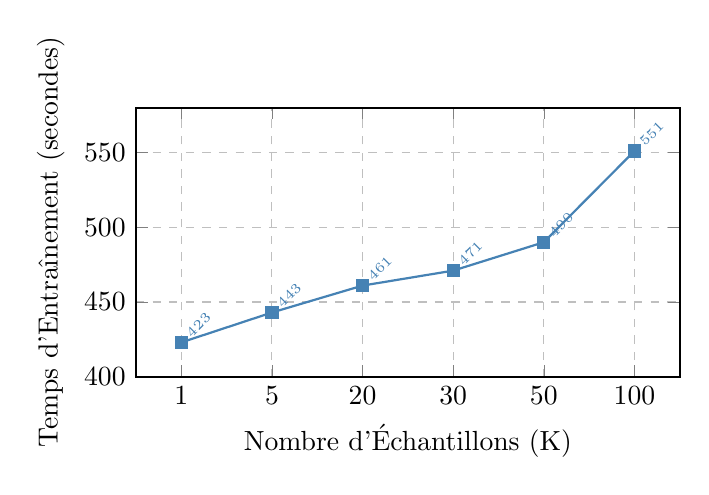
\begin{tikzpicture}
        \begin{axis}[
            width=0.7\textwidth,
            height=5cm,
            xlabel={Nombre d'Échantillons (K)},
            ylabel={Temps d'Entraînement (secondes)},
            symbolic x coords={1, 5, 20, 30, 50, 100},
            xtick=data,
            ymin=400,
            ymax=580,
            nodes near coords,
            every node near coord/.append style={font=\tiny, rotate=45, anchor=west},
            mark=*,
            thick,
            grid=major,
            grid style=dashed,
        ]
        \addplot[color=myBlue, mark=square*, thick] coordinates {
            (1, 423)
            (5, 443)
            (20, 461)
            (30, 471)
            (50, 490)
            (100, 551)
        };
        \end{axis}
    \end{tikzpicture}
    \caption{Temps d'Entraînement vs. Nombre d'Échantillons}
    \label{fig:trainingtime}
\end{figure}

Le temps d'entraînement évolue de manière \textbf{sous-linéaire} avec $K$ grâce au calcul parallèle efficace sur GPU. Le surcoût de $K=1$ à $K=100$ est d'environ 30\%, un coût raisonnable pour les améliorations significatives du serrage de la borne.

\subsection{Qualité des Échantillons}

La comparaison visuelle des échantillons générés montre que l'IWAE produit des reconstructions plus nettes avec des traits plus définis, tandis que les échantillons du VAE tendent à apparaître plus flous et moyennés.

% ---------------------------------------------------------
\section{Résumé des Compromis}

\begin{table}[h]
    \centering
    \begin{tabular}{l|c|c}
        \toprule
        \textbf{Métrique} & \textbf{VAE (K=1)} & \textbf{IWAE (K=50)} \\
        \midrule
        Serrage de la Borne & Lâche & \textbf{Serrée} \\
        Utilisation Latente & Risque d'Effondrement & \textbf{Riche (35/50)} \\
        Variance de la Borne & Élevée & \textbf{Faible} \\
        SNR Gradient Encodeur & \textbf{Élevé} & Faible \\
        Qualité des Échantillons & Flous & \textbf{Nets} \\
        Coût de Calcul & \textbf{Faible} & Élevé ($\times K$) \\
        \bottomrule
    \end{tabular}
    \caption{Comparaison des compromis VAE et IWAE}
    \label{tab:tradeoffs}
\end{table}

% ---------------------------------------------------------
\section{Recherches Récentes sur l'IWAE}

Depuis l'article original sur l'IWAE \cite{burda2015importance}, des recherches significatives ont abordé ses limitations et étendu ses applications.

\subsection{Adresser le Problème du SNR}

Plusieurs techniques ont été proposées pour atténuer la dégradation du SNR du gradient de l'encodeur :

\textbf{IWAE-STL (Sticking the Landing)} \cite{roeder2017sticking} : Cette approche supprime le terme de fonction de score du gradient, réduisant la variance et améliorant la stabilité de l'entraînement de l'encodeur.

\textbf{IWAE-DREG (Doubly Reparameterized Gradient Estimators)} \cite{tucker2019doubly} : Tucker et al. ont proposé un estimateur doublement reparamétrisé qui fournit des gradients non biaisés avec une variance plus faible pour le réseau d'inférence. Cette approche a montré une amélioration du SNR pour les composants encodeur et décodeur.

\textbf{VR-IWAE} \cite{daudel2024learning} : Daudel et al. (2024) ont analysé le comportement asymptotique des estimateurs reparamétrisés et doublement reparamétrisés lorsqu'ils sont appliqués à l'objectif VR-IWAE. Leur travail montre que pour des valeurs spécifiques du paramètre variationnel de Rényi $\alpha$, le SNR évolue favorablement avec à la fois le nombre d'estimations indépendantes $M$ et les échantillons d'importance $N$.

\subsection{Variantes de l'IWAE}

\textbf{MIWAE (Missing Data IWAE)} \cite{mattei2019miwae} : Étend l'IWAE pour gérer l'imputation de données manquantes en traitant les valeurs manquantes comme des variables latentes.

\textbf{CIWAE (Combination IWAE)} \cite{huang2019ciwae} : Propose une combinaison convexe des objectifs VAE et IWAE pour équilibrer le compromis entre des bornes plus serrées et de meilleurs gradients pour l'encodeur.

\textbf{IWAE Récursif} \cite{brekelmans2024recursive} : Des travaux récents (2024) explorent l'apprentissage récursif d'objectifs variationnels asymptotiques, étendant le cadre IWAE pour atteindre des bornes plus serrées grâce à l'échantillonnage préférentiel imbriqué.

\subsection{Avancées Théoriques}

\textbf{Sur le paradoxe de la borne plus serrée :} \citet{rainforth2018tighter} ont fourni une analyse rigoureuse montrant que des bornes plus serrées ne sont pas toujours meilleures pour l'apprentissage. Leur travail formalise le phénomène de dégradation du SNR et suggère que des valeurs intermédiaires de $K$ peuvent être optimales.

\textbf{Prévention de l'Effondrement du Postérieur :} Des travaux récents tels que Scale-VAE \cite{scalevae2024} continuent d'aborder le problème d'effondrement du postérieur que tant le VAE que l'IWAE visent à résoudre, suggérant un intérêt continu pour un apprentissage robuste de l'espace latent.

% ---------------------------------------------------------
\section{Conclusion}

L'Importance Weighted Autoencoder fournit une approche rigoureuse pour atteindre des bornes plus serrées sur la log-vraisemblance tout en apprenant des représentations latentes plus riches. Nos expériences sur MNIST confirment les prédictions théoriques : augmenter $K$ améliore l'estimation de la log-vraisemblance et augmente l'utilisation de l'espace latent.

Cependant, l'IWAE n'est pas sans inconvénients. Le rapport signal sur bruit pour les gradients de l'encodeur diminue avec $K$, créant une asymétrie où le décodeur bénéficie davantage des échantillons supplémentaires que l'encodeur. Cela suggère que les praticiens devraient choisir soigneusement $K$ en fonction de leurs besoins spécifiques, utilisant potentiellement des techniques comme DREG ou CIWAE pour atténuer le problème d'apprentissage de l'encodeur.

Les travaux futurs pourraient explorer des méthodes adaptatives qui ajustent dynamiquement $K$ pendant l'entraînement, ou des approches hybrides qui combinent les avantages de bornes serrées avec des gradients stables pour l'encodeur.

% ---------------------------------------------------------
% REFERENCES
% ---------------------------------------------------------
\bibliographystyle{plain}
\begin{thebibliography}{99}

\bibitem{kingma2013auto}
Kingma, D.P. et Welling, M. (2013).
\newblock Auto-Encoding Variational Bayes.
\newblock {\em arXiv preprint arXiv:1312.6114}.

\bibitem{burda2015importance}
Burda, Y., Grosse, R., et Salakhutdinov, R. (2015).
\newblock Importance Weighted Autoencoders.
\newblock {\em arXiv preprint arXiv:1509.00519}.

\bibitem{rainforth2018tighter}
Rainforth, T., Kosiorek, A.R., Le, T.A., Maddison, C.J., Igl, M., Wood, F., et Teh, Y.W. (2018).
\newblock Tighter Variational Bounds are Not Necessarily Better.
\newblock {\em International Conference on Machine Learning (ICML)}.

\bibitem{roeder2017sticking}
Roeder, G., Wu, Y., et Duvenaud, D. (2017).
\newblock Sticking the Landing: Simple, Lower-Variance Gradient Estimators for Variational Inference.
\newblock {\em Advances in Neural Information Processing Systems (NeurIPS)}.

\bibitem{tucker2019doubly}
Tucker, G., Lawson, D., Gu, S., et Maddison, C.J. (2019).
\newblock Doubly Reparameterized Gradient Estimators for Monte Carlo Objectives.
\newblock {\em International Conference on Learning Representations (ICLR)}.

\bibitem{daudel2024learning}
Daudel, K., Guérin, J., et Moulines, E. (2024).
\newblock Learning with Importance Weighted Variational Inference: Asymptotics for Gradient Estimators of the VR-IWAE Bound.
\newblock {\em arXiv preprint}.

\bibitem{mattei2019miwae}
Mattei, P.A. et Frellsen, J. (2019).
\newblock MIWAE: Deep Generative Modelling and Imputation of Incomplete Data Sets.
\newblock {\em International Conference on Machine Learning (ICML)}.

\bibitem{huang2019ciwae}
Huang, C.W. et Wu, C. (2019).
\newblock CIWAE: Convex Combinations of IWAE and VAE.
\newblock {\em NeurIPS Workshop on Bayesian Deep Learning}.

\bibitem{brekelmans2024recursive}
Brekelmans, R. et al. (2024).
\newblock Recursive Learning of Asymptotic Variational Objectives.
\newblock {\em International Conference on Machine Learning (ICML)}.

\bibitem{scalevae2024}
Zhang, X. et al. (2024).
\newblock Scale-VAE: Preventing Posterior Collapse in Variational Autoencoder.
\newblock {\em arXiv preprint}.

\end{thebibliography}

\end{document}